\chapter{BaseLib Level 2}
\chaptermark{Level 2}

%andre articolo
A series of classes are dedicated to strings and data streaming. These allow to perform a series of advanced operations in character sequences and to perform input/output (I/O) operations without requiring the concept of beginning and end of transmission. Most of the I/O classes are abstracted to a level where the knowledge of the target media (socket, memory, ...) isn't required. Such classes come from BaseLib Level 2 and inherits from \texttt{level0::StreamInterface} and its implementation \texttt{level2::Streamable}.\\


The main concept in this chapter is the \texttt{Streamable} class that is presented before every other class.
As usual we discuss each section in a logical order; Level2 asa said before implements the concept of stream, a common concept in C++ and in Java, slighty new to C programmers that are used to work with files, sockets or strings. All this concepts are groupped togheter and are accesible via the \texttt{level0::StreamInterface}. \texttt{Streamable} implements \texttt{StreamInterface} and adds some metods and attributes.\\


Analysis is carried on examining the differents stream object grouped in two sets: memory (buffer, string handling) and files (also sockets that are no more than files in Unix view). The whole BaseLib Level 2 could be divided in the following sections:
\begin{itemize}
 \item Streamable (memory, files)
 \item CDB
 \item IO devices (serial line, keyboard)
\end{itemize}



\section{Streamable}
Before reading this section is really important that one has read \textit{BaseLib} \textit{Level0} \textit{Streams} section. Such a section introduces streams and the \texttt{StreamInterface} from which the \texttt{Streamable} inherits from. This section treats first the class \texttt{Streamable} and then we have a look first to memory streams and then to file streams. We take a look first to memory streams because there is an important class on which the \texttt{Streamable} class relies on. To have a pictorial idea of the \texttt{Streamable} class introduced below refer to Figure \ref{f:level2:stream_mem} and Figure \ref{f:level2:stream_file}.



\subsubsection{Streamable}
\texttt{[Streamable.h, Streamable.cpp]}\\
Most of the methods in \texttt{Streamable} class are an implementation of what is simply declared in the \texttt{StreamInterface} class in Level0. \texttt{Streamable} is the prototype for all streams, it adds to StreamInterface some buffering and token searching functions.\\


The class \texttt{Streamable} relies on the \texttt{CStreamBuffering} class described in the following sections, of such type are the first two attributes, the first is the \textit{input} buffering area and the second is the \textit{output} buffering area (\texttt{csbIn} and \texttt{csbOut}). Last attribute is a stream identifier, if hold the value \texttt{0} means the default stream and if is \texttt{-1} it means no stream.

The constructor simply set to \texttt{NULL} each attribute and the destructor does nothing.
\begin{lstlisting}[
extendedchars=true,%
basicstyle=\fontfamily{pcr}\fontseries{m}\selectfont\footnotesize, %
stepnumber=1,%
numberstyle=\tiny,%
keywordstyle=\footnotesize\tt ,%
language=C++]
protected:
   CStreamBuffering* csbIn;
   CStreamBuffering* csbOut;
   uint32 selectedStream;
public:
   Streamable();
   virtual ~Streamable();
\end{lstlisting}

The first two methods we encounter, \texttt{SSRead} and \texttt{SSWrite} are two virtual methods not implemented here but to be implemented by any subclass. \texttt{CanRead} and \texttt{CanWrite} simply return \texttt{False} because methods \texttt{SSRead}, \texttt{SSWrite} are not implemented for the class. Methods \texttt{Read} and \texttt{GetC} call \texttt{SSRead}; methods \texttt{Write} and \texttt{PutC} call \texttt{SSWrite}.
\begin{lstlisting}[
extendedchars=true,%
basicstyle=\fontfamily{pcr}\fontseries{m}\selectfont\footnotesize, %
stepnumber=1,%
numberstyle=\tiny,%
keywordstyle=\footnotesize\tt ,%
language=C++]
protected:
   virtual bool SSRead(void* buffer,uint32& size,TimeoutType msecTimeout=TTDefault)=0;
   virtual bool SSWrite(const void* buffer,uint32& size,TimeoutType msecTimeout=TTDefault)=0;

public:
   virtual bool Read(void* buffer,uint32& size,TimeoutType msecTimeout=TTDefault);
   virtual bool Write(const void* buffer,uint32& size,TimeoutType msecTimeout=TTDefault);

   virtual bool CanRead();
   virtual bool CanWrite();

   inline bool GetC(char& c);
   inline bool PutC(char c);
\end{lstlisting}

The method \texttt{Size} must return the size of the file, in this case it will return\texttt{-1} because \texttt{Streamable} is an abstract class; the same happens for the method \texttt{Position}. Methods \texttt{SetSize}, \texttt{Seek} and \texttt{CanSeek} return \texttt{False}. All those methods must be implemented in a subclass. \\


The method \texttt{NOfStreams} return \texttt{1}, such method return how many streams are available, override it with a different value if multiple stream are supported. The first \texttt{Switch} method select the stream to read from, switching may reset the stream to the start, \texttt{0} is the default stream, \texttt{false} is only returned if the switch was not performed. Also the second \texttt{Switch} selects the stream to read from, must be overriden with a method providing name to number mapping. The method \texttt{SelectedStream} returns what stream has been selected and \texttt{StreamName} returns the name of the stream we are using.
The method \texttt{AddStream} adds a new stream to write in and \texttt{RemoveStream} removes an existing stream. Those last two methods are not implemented in this class and return \texttt{false}.\\


The method \texttt{CompleteRead} performs the job of a the read function but guarantees the completion; in case of failure, \texttt{size} returns the actual data read; \texttt{timeOutMs} is the total allowed wait time checked using \texttt{level0::HRT}. The method \texttt{CompleteWrite} performs the job of a write function but guarantees the completion; in case of failure size returns the actual data written; those functions are implemented in the \textit{Streamable.cpp} file.
\begin{lstlisting}[
extendedchars=true,%
basicstyle=\fontfamily{pcr}\fontseries{m}\selectfont\footnotesize, %
stepnumber=1,%
numberstyle=\tiny,%
keywordstyle=\footnotesize\tt ,%
language=C++]
   virtual int64 Size();
   virtual bool SetSize(int64 size);
   virtual int64 Position(void);
   virtual bool Seek(int64 pos);
   virtual bool CanSeek();

   virtual uint32 NOfStreams();
   virtual bool Switch(uint32 selectedStream);
   virtual bool Switch(const char* name);
   virtual uint32 SelectedStream();
   virtual bool StreamName(uint32 n,char* name,int nameSize);
   virtual bool AddStream(const char* name);
   virtual bool RemoveStream(const char *name);

   virtual bool CompleteRead(void* buffer,uint32& size,
      TimeoutType msecTimeout = TTInfiniteWait);
   virtual bool CompleteWrite(const void* buffer,uint32& size,
      TimeoutType msecTimeout = TTInfiniteWait);
\end{lstlisting}

Now we introduce three functions firstly implemented in the \texttt{Streamable} class, those function make use of the attributes in the \texttt{Streamable} class.

The method \texttt{BufferedRead} writes the buffer from the stream; it's better to not remap this function unless the class needs to deal with buffering in a different way.
The method \texttt{BufferedWrite} reads and copies data into the stream; it is important to not remap this function unless the class needs to deal with buffering in a different way, like the previous method. \texttt{Flush} forces to complete buffered operations.
\begin{lstlisting}[
extendedchars=true,%
basicstyle=\fontfamily{pcr}\fontseries{m}\selectfont\footnotesize, %
stepnumber=1,%
numberstyle=\tiny,%
keywordstyle=\footnotesize\tt ,%
language=C++]
   virtual bool BufferedRead(void* buffer,uint32& size,
      TimeoutType msecTimeout = TTDefault);
   virtual bool BufferedWrite(const void* buffer,uint32& size,
      TimeoutType msecTimeout = TTDefault);
   inline void Flush();
\end{lstlisting}

The method \texttt{VPrintf} will write any text using printf format (is buffered if buffering is activated), the others \texttt{Print} functions print, respectively, an integer, a flot or a string with desidered size and padding to the output stream registered with the \texttt{Streamable} class (attribute \texttt{csbOut}).
\begin{lstlisting}[
extendedchars=true,%
basicstyle=\fontfamily{pcr}\fontseries{m}\selectfont\footnotesize, %
stepnumber=1,%
numberstyle=\tiny,%
keywordstyle=\footnotesize\tt ,%
language=C++]
   bool VPrintf(const char* format,va_list argList);
   inline bool Print(int32 n,int desiredSize=0,
      char desiredPadding=0,char mode = 'i');
   inline bool Print(double f,int desiredSize=0,
      int desiredSubSize=6,char desiredPadding=0,char mode='f');
   inline bool Print(const char* s,int desiredSize=0,
      char desiredPadding=0);
\end{lstlisting}


First \texttt{GetToken} method extracts a token from the stream into a string data until a terminator or 0 is found; \texttt{maxSize} is the buffer size, the maximum string size is \texttt{maxSize-1}; it skips all \texttt{skipCharacters} chars even if calssified also as terminators if at the beginning returns \texttt{true} if some data was read before any error or file termination. \texttt{false} only on error and no data available; the terminator (just the first encountered) is consumed in the process and saved in \texttt{saveTerminator} if provided. This is a buffered method.
Second \texttt{GetToken} method behave in the same way as before but takes as the first argument an \texttt{StreamInterface} object. A character can be found in the terminator or in the \texttt{skipCharacters} list in both or in none. See Table \ref{t:level2:gettoken} for an explanation on how it work. The same things can be said for the third \texttt{GetToken} but it takes a string as a \texttt{Streamable} reference.

\begin{table}[!h]
 \begin{center}
  \begin{tabular}{|l|l|}
   \hline
    \textbf{char in} & \textbf{action preformed} \\
   \hline
    none & the character is copied \\
    terminator & the character is not copied the string is terminated \\
    skip & the character is not copied \\
    skip and terminator & the character is not copied, the string is terminated if not empty \\
   \hline
   \end{tabular}
   \end{center}
  \caption{Level2 GetToken actions}
 \label{t:level2:gettoken}
\end{table}

\texttt{SkipTokens} skips a series of tokens delimited by terminators or 0.
\texttt{GetLine} will skip an empty line or any part of a line termination (the first working on a \texttt{Streamable} input and the second on a \texttt{char*} input extracting the substring after skipping the required line). \\


Next two methods are \texttt{static}, the first one \texttt{GetCStringToken} extracts a token from the string into a string until a terminator or 0 is found, the maximum string size is $maxSize-1$, it returns \texttt{true} if some data was read. False only on no data available. The method \texttt{DestructiveGetCStringToken} extracts a token from the string into a string until a terminator or 0 is found and affects the input by placing 0 at the end of each token.\\


Last method, \texttt{FindPattern} extracts data from the stream until the matching string is found the pointer is to the first character after the pattern.
\begin{lstlisting}[
extendedchars=true,%
basicstyle=\fontfamily{pcr}\fontseries{m}\selectfont\footnotesize, %
stepnumber=1,%
numberstyle=\tiny,%
keywordstyle=\footnotesize\tt ,%
language=C++]
   virtual bool GetToken(char* buffer,const char* terminator,
      uint32 maxSize,char* saveTerminator=NULL,const char* skipCharacters=NULL);
   virtual bool GetToken(StreamInterface& output,const char* terminator,
      char* saveTerminator=NULL,const char* skipCharacters=NULL);
   virtual bool GetToken(Streamable& output,const char* terminator,
      char* saveTerminator=NULL,const char* skipCharacters=NULL);

   virtual bool SkipTokens(uint32 count, const char* terminator);
   virtual bool GetLine(Streamable& output, bool skipTerminators=True);
   virtual bool GetLine(char* buffer,uint32 maxSize,bool skipTerminators=True);

   static inline bool GetCStringToken(const char*& input,char* buffer,
      const char* terminator,uint32 maxSize);
   static inline char* DestructiveGetCStringToken(char*& input,const char* terminator,
      char* saveTerminator=NULL,const char* skipCharacters="");

   inline bool FindPattern(const char *pattern);
\end{lstlisting}



\subsection{Memory Streams}
Memory streams are all streams involving memory operations like strings and buffers. All classes that depend on this group are depicted in the UML diagram of Figure \ref{f:level2:stream_mem}.
\begin{figure}[h!]
 \begin{center}
  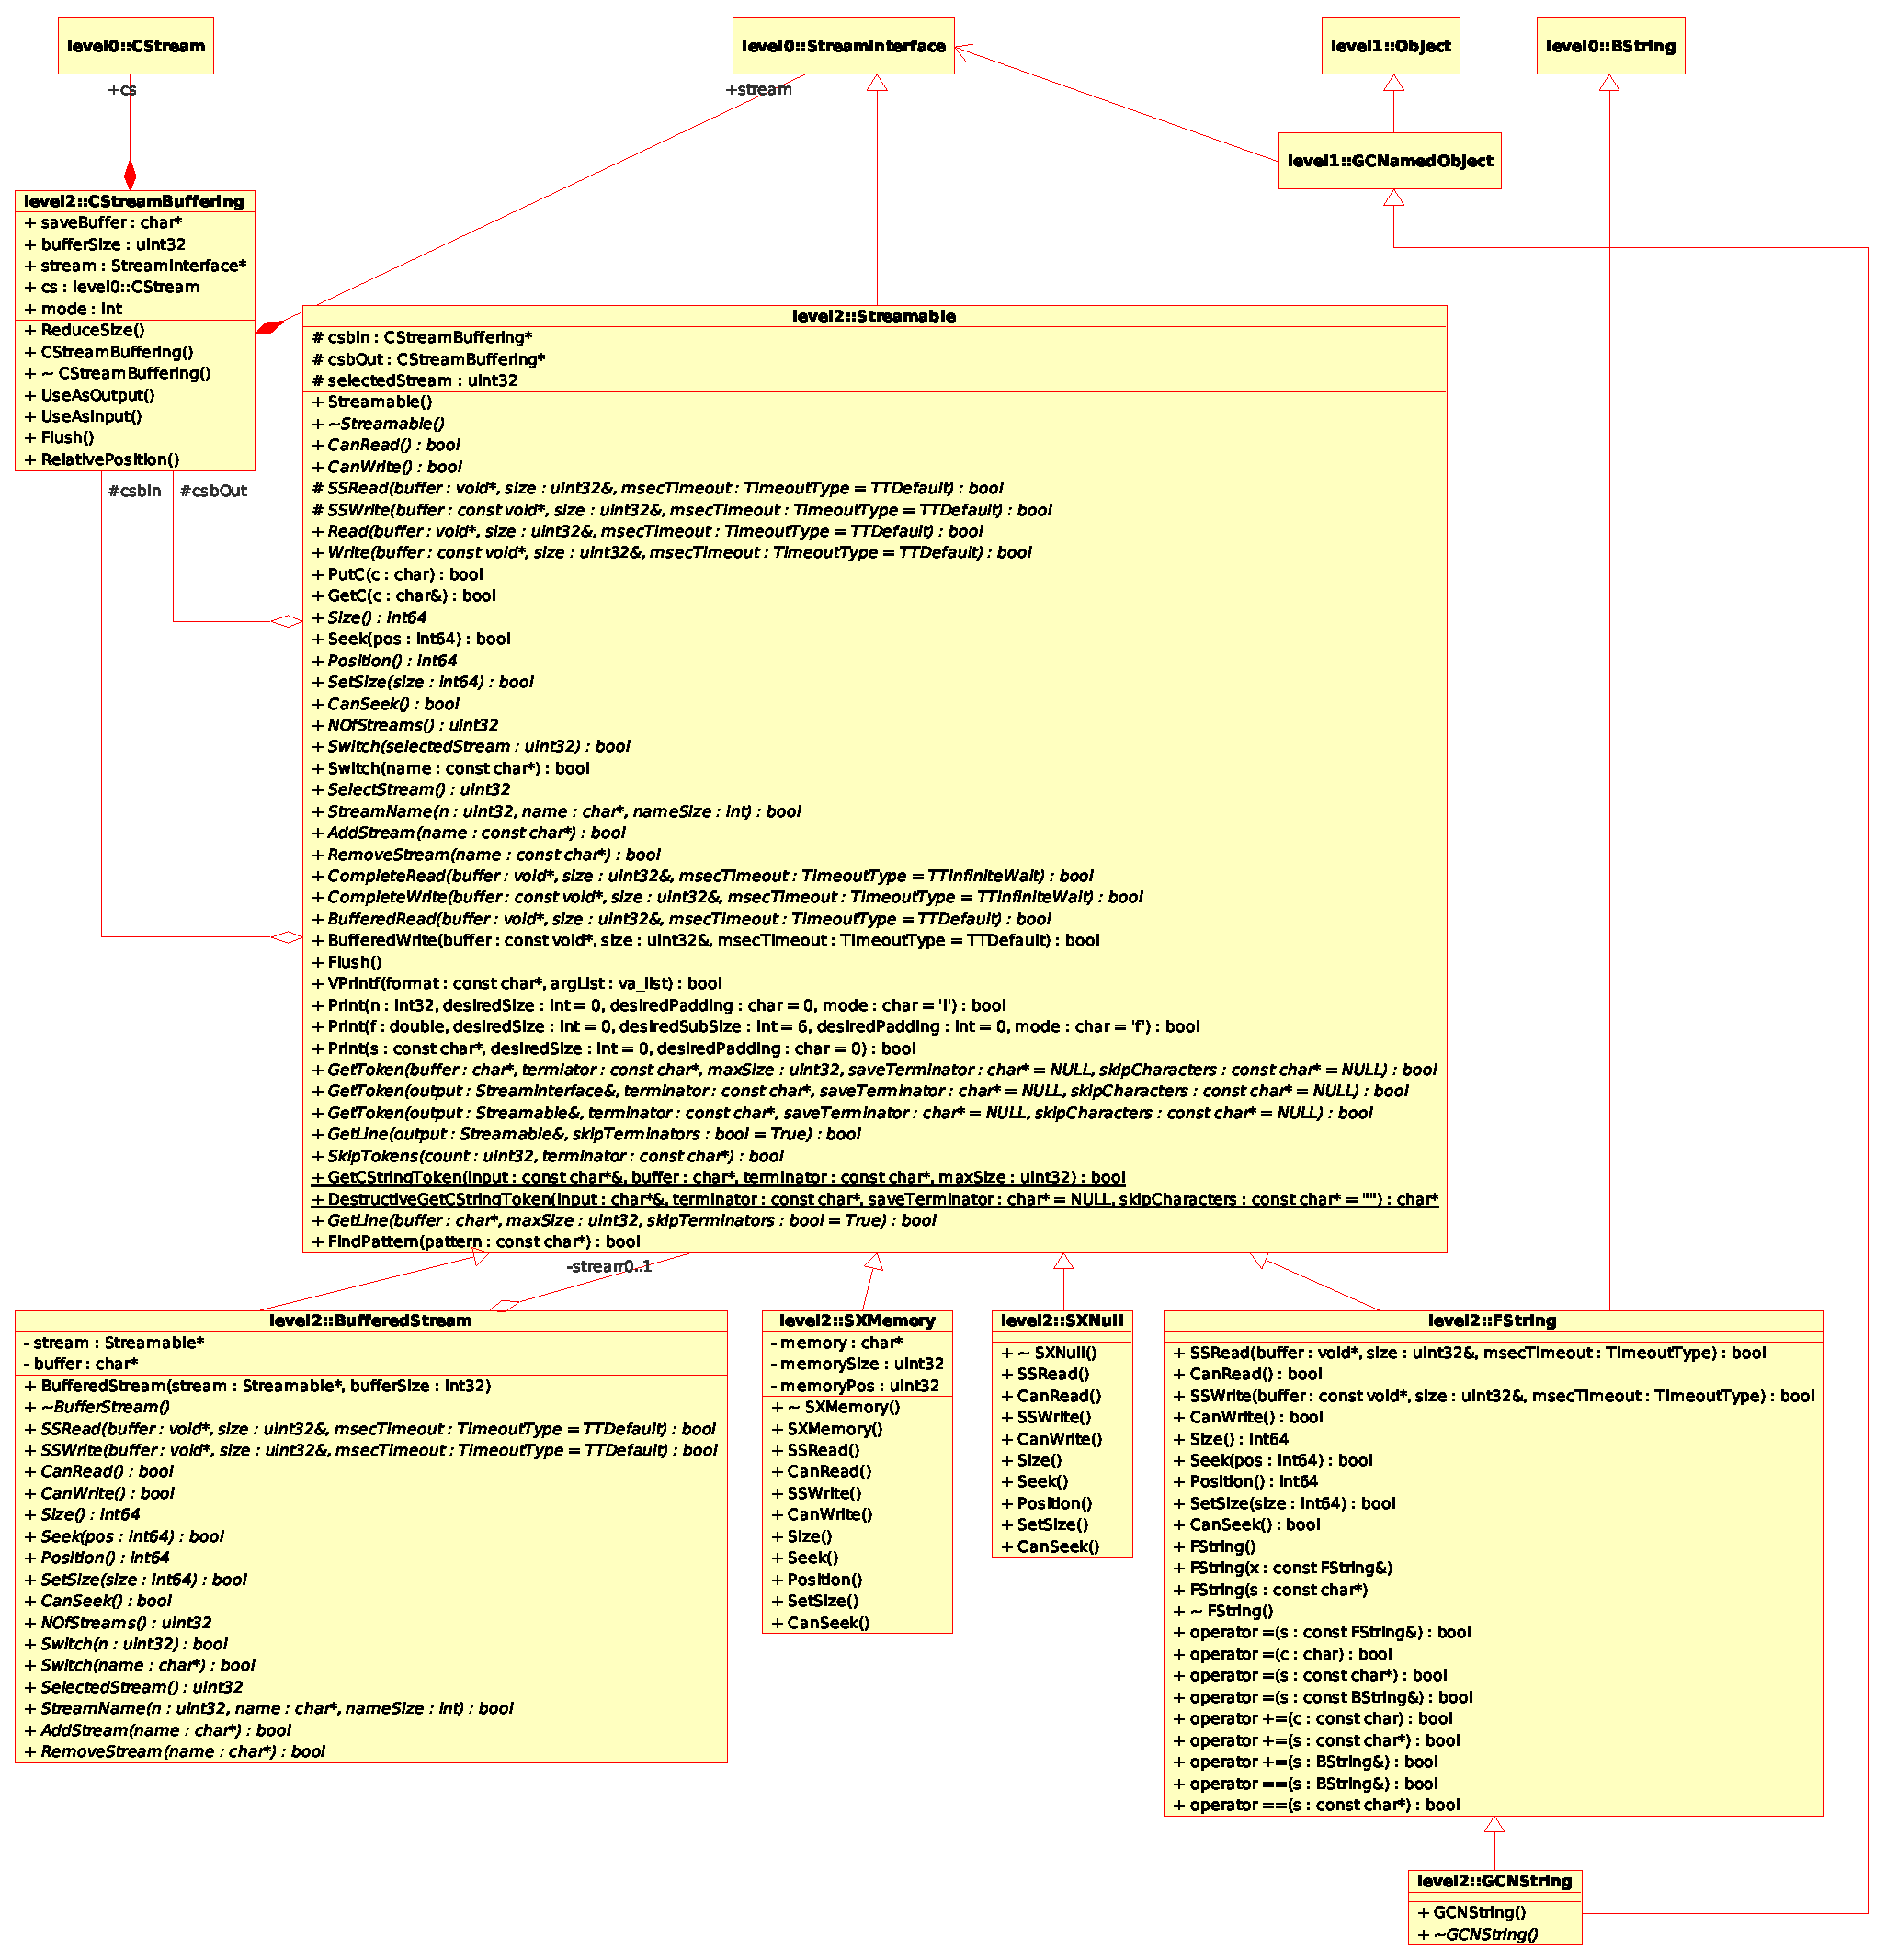
\includegraphics[width=\textwidth]{level2/level2-mstream.eps}
  \caption{BaseLib Level2 memory stream classes}
  \label{f:level2:stream_mem}
 \end{center}
\end{figure}

Class involved are listed below. Most of the classes are quite similar, the only notable difference is the \texttt{CStreamBuffering} class that is not a subclass of the \texttt{Streamable} class. We start analysing this class.
\begin{itemize}
 \item CStreamBuffering
 \item BufferedStream
 \item SXMemory, SXNull
 \item FString, GCNString
\end{itemize}



\subsubsection{CStreamBuffering}
\texttt{[CStreamBuffering.h, CStreamBuffering.cpp]}\\
This class basically maps a \texttt{StreamInterface} to a \texttt{CStream} class providing buffering to the \texttt{CStream}.

The class has infact as attributes a \texttt{StreamInterface} pointer and a \texttt{CStream}. The constructor let the user set those attributes. The working mode, attribute \texttt{mode}, can be set with \texttt{UseAsOutput} and \texttt{UseAsInput}.
\begin{lstlisting}[
extendedchars=true,%
basicstyle=\fontfamily{pcr}\fontseries{m}\selectfont\footnotesize, %
stepnumber=1,%
numberstyle=\tiny,%
keywordstyle=\footnotesize\tt ,%
language=C++]
public:
   char* saveBuffer;
   uint32 bufferSize;
   StreamInterface* stream;
   CStream cs;
   int mode;
public:
   CStreamBuffering(StreamInterface* stream,char* buffer,int bufferSize);
   virtual ~CStreamBuffering();

   void ReduceSize(int bufferSize);
   CStream* UseAsOutput();
   CStream* UseAsInput();
   void Flush();
   int32 RelativePosition();
\end{lstlisting}



\subsubsection{BufferedStream}
\texttt{[BufferedStream.h, BufferedStream.cpp]}\\
Class \texttt{BufferedStream} provides full buffering support to a \texttt{Streamable} class by wrapping the non buffering functions. Those functions are basically the \texttt{Streamable} protected \texttt{SSRead} and \texttt{SSWrite}.\\


To buffer a \texttt{Streamable} it has attributes a \texttt{Streamable} and a \texttt{char*} that will be the buffering area. The constructor require a \texttt{Streamable} that will be firtly saved in the associated attribute and then buffered, the buffering area will be required via the argument \texttt{bufferSize}. Take care because the constructor if initialized with a \texttt{NULL} \texttt{Streamable} pointer will exit without creating a valid object.

\begin{lstlisting}[
extendedchars=true,%
basicstyle=\fontfamily{pcr}\fontseries{m}\selectfont\footnotesize, %
stepnumber=1,%
numberstyle=\tiny,%
keywordstyle=\footnotesize\tt ,%
language=C++]
private:
   Streamable* stream;
   char* buffer;
public:
   BufferedStream(Streamable* stream,int32 bufferSize);
   virtual ~BufferedStream();
\end{lstlisting}

This not so difficult implementation in \texttt{SSRead} and \texttt{SSWrite} call \texttt{BufferedRead} and \texttt{BufferedWrite} on the saved \texttt{Streamable} attribute to achieve buffered operations.

All other methods call the respective method of the saved \texttt{Streamable} attribute.
\begin{lstlisting}[
extendedchars=true,%
basicstyle=\fontfamily{pcr}\fontseries{m}\selectfont\footnotesize, %
stepnumber=1,%
numberstyle=\tiny,%
keywordstyle=\footnotesize\tt ,%
language=C++]
   virtual bool SSRead(void* buffer,uint32& size,TimeoutType msecTimeout=TTDefault);
   virtual bool SSWrite(const void* buffer,uint32& size,TimeoutType msecTimeout=TTDefault);
   virtual bool CanRead();
   virtual bool CanWrite();

   virtual int64 Size();
   virtual bool  Seek(int64 pos);
   virtual int64 Position(void);
   virtual bool  SetSize(int64 size);
   virtual bool  CanSeek();

   virtual uint32 NOfStreams();
   virtual bool Switch(uint32 n);
   virtual bool Switch(const char* name);
   virtual uint32 SelectedStream();
   virtual bool StreamName(uint32 n,char* name,int nameSize);
   virtual bool AddStream(const char* name);
   virtual bool RemoveStream(const char* name);
\end{lstlisting}



\subsubsection{SXMemory, SXNull}
\texttt{[SXMemory.h, SXNull.h]}\\
The class \texttt{SXMemory} is a \textit{Streamable eXtension Memory} for a buffer; i.e.it provides read and write operation from/to a buffer in memory. With this class it is possible to use a piece of memory user allocated like a stream.\\


The memory to be used must be previously allocated and then, you have to use the obtained pointer as an argument to the class's constructor. The constructor doesn't check for arguments consistency and simply store the arguements in the attributes. \texttt{memoryPos} will be set to zero.
\begin{lstlisting}[
extendedchars=true,%
basicstyle=\fontfamily{pcr}\fontseries{m}\selectfont\footnotesize, %
stepnumber=1,%
numberstyle=\tiny,%
keywordstyle=\footnotesize\tt ,%
language=C++]
   char* memory;
   uint32 memorySize;
   uint32 memoryPos;
public:
   SXMemory(char* mem,uint32 size);
   virtual ~SXMemory();
\end{lstlisting}

Also in this class the main methods are \texttt{SSRead} and \texttt{SSWrite} that mainly make use of \texttt{memcpy} to do its work. Other methods are straightforward.
\begin{lstlisting}[
extendedchars=true,%
basicstyle=\fontfamily{pcr}\fontseries{m}\selectfont\footnotesize, %
stepnumber=1,%
numberstyle=\tiny,%
keywordstyle=\footnotesize\tt ,%
language=C++]
   virtual bool SSRead(void* buffer,uint32& size,TimeoutType msecTimeout=TTDefault);
   virtual bool SSWrite(const void* buffer,uint32& size,TimeoutType msecTimeout=TTDefault);
   virtual bool CanRead();
   virtual bool CanWrite();

   virtual int64 Size();
   virtual bool Seek(int64 pos);
   virtual int64 Position(void);
   virtual bool SetSize(int64 size);
   virtual bool CanSeek();
\end{lstlisting}

Like you can see in the UML diagram of Figure \ref{f:level2:stream_memS} there is also a class \texttt{SXNull} who's name stand for \textit{Streamable eXtension Null} that is a null or no stream class, so it not implement any stream but is a dummy one.



\subsubsection{FString, GCNString}
\texttt{[FString.h, FString.cpp, GCNString.h, GCNString.cpp]}\\
The class \texttt{FString} extends \texttt{BString} and \texttt{Streamable} and concretely is a class containing a string simulating a file, or better a streamable interface of a string. Reading a and writing are done on a specific position.\\


It holds no attributes and implements, like in the previous classes, protected \texttt{SSRead} and \texttt{SSWrite} methods. Strings operator concatenation and copy are overridden.
\begin{lstlisting}[
extendedchars=true,%
basicstyle=\fontfamily{pcr}\fontseries{m}\selectfont\footnotesize, %
stepnumber=1,%
numberstyle=\tiny,%
keywordstyle=\footnotesize\tt ,%
language=C++]
public:
   virtual bool SSRead(void* buffer,uint32& size,TimeoutType msecTimeout=TTDefault);
   virtual bool SSWrite(const void* buffer,uint32& size,TimeoutType msecTimeout=TTDefault);
   virtual bool CanRead();
   virtual bool CanWrite();

   virtual int64 Size();
   virtual bool Seek(int64 pos);
   virtual int64 Position(void);
   virtual bool SetSize(int64 size);
   virtual bool CanSeek();

   FString();
   FString(const FString& x);
   FString(const char* s);
   virtual ~FString();

   inline bool operator=(const FString& s);
   inline bool operator=(char c);
   inline bool operator=(const char* s);
   inline bool operator=(const BString& s);
   inline bool operator+=(const char c);
   inline bool operator+=(const char* s);
   inline bool operator+=(BString& s);
   inline bool operator==(BString& s) const;
   inline bool operator==(const char* s) const;
\end{lstlisting}

The class \texttt{GCNString} is an \texttt{FString} with a \texttt{GCNamedObject} parenthood. The class implements no further methods.



\subsection{File Streams}
File streams are all streams involving file operations. File operations are intended in the UNIX way, i.e. for example in UNIX sockets but also console are files. All classes that depend on this group are depicted in the UML diagram of Figure \ref{f:level2:stream_file}.
\begin{figure}[h!]
 \begin{center}
  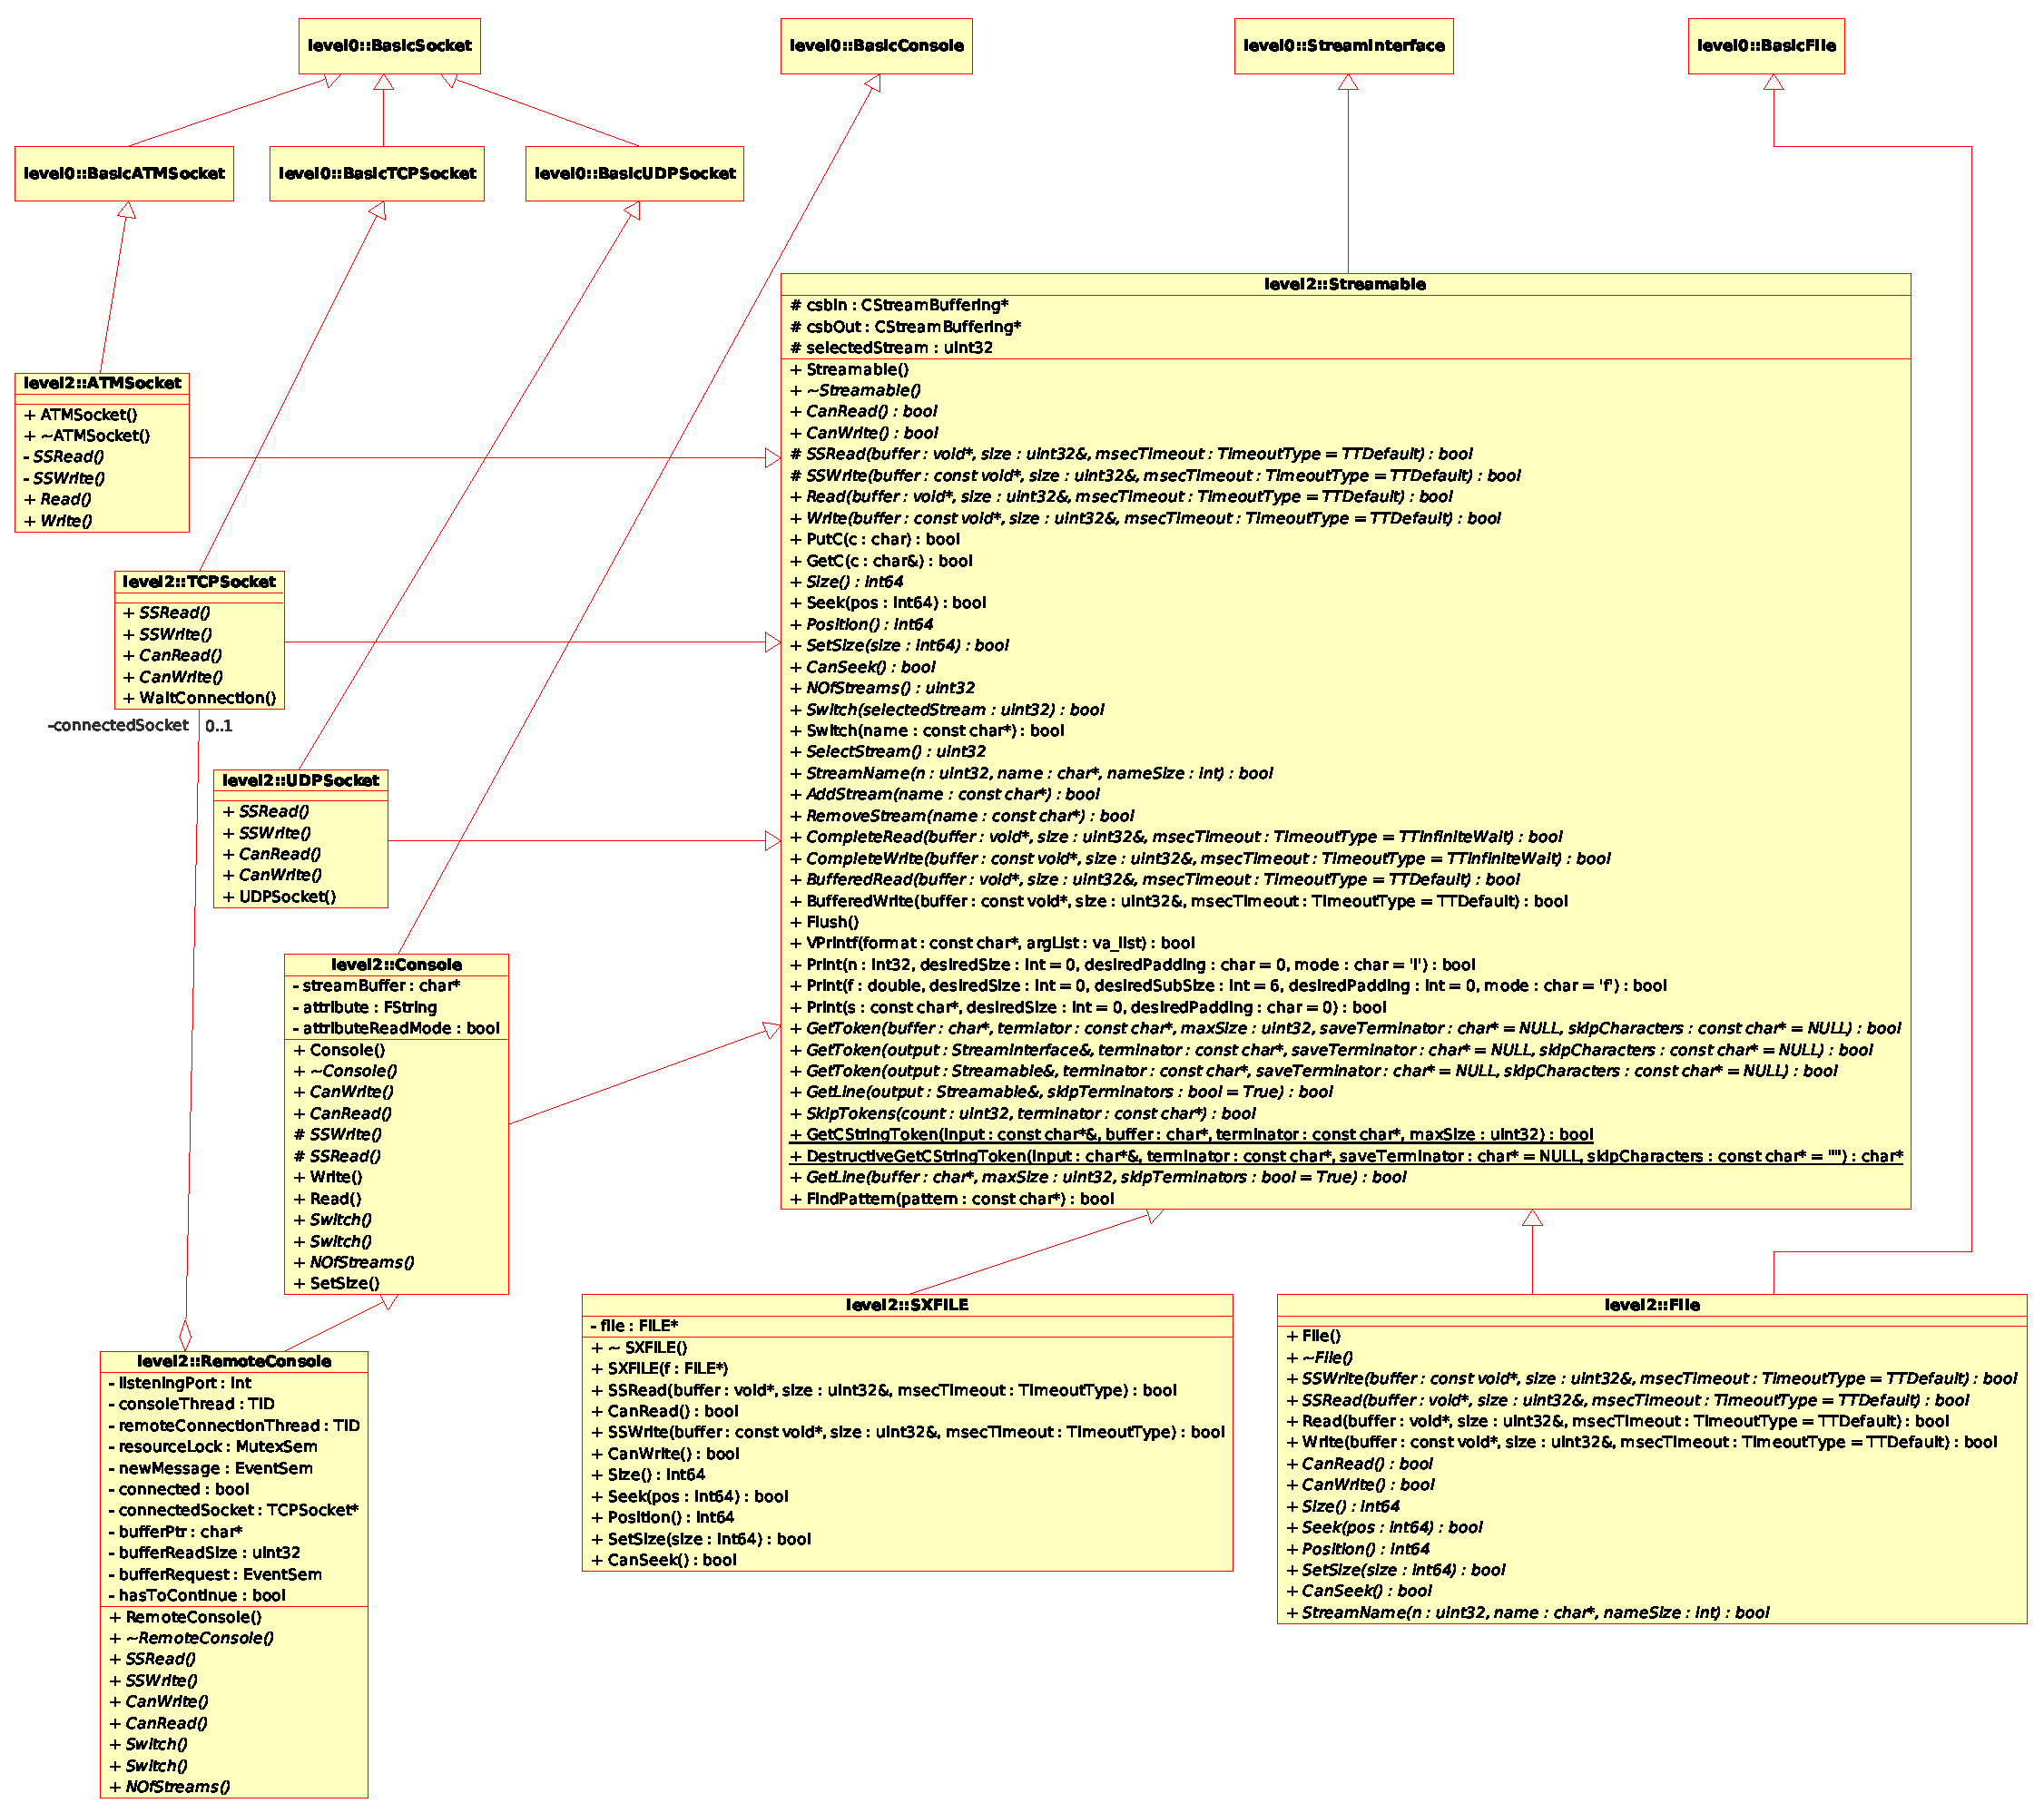
\includegraphics[width=\textwidth]{level2/level2-fstream.eps}
  \caption{BaseLib Level2 file streams classes}
  \label{f:level2:stream_file}
 \end{center}
\end{figure}

Class involved are listed below. Most of the classes are quite similar, classes can be groupped in three subcategories: network (sockets), console and file. But we doesn't follow this distintiction.
\begin{itemize}
 \item ATMSocket
 \item TCPSocket
 \item UDPSocket

 \item Console
 \item RemoteConsole

 \item File
 \item SXFILE
\end{itemize}



\subsubsection{ATMSocket}
\texttt{[ATMSocket.h, ATMSocket.cpp]}\\
The class \texttt{ATMSocket} adds the streamable capability to a \texttt{BasicATMSocket}, i.e. a \texttt{BasicATMSocket} can also be treat as a stream of data. In detail such class implements ATM sockets AAL5 layer.\\


The method \texttt{SSRead} reads a block of data from the socket, \texttt{size} is the maximum size, on return \texttt{size} is what was read, timeout is not supported yet. The method \texttt{SSWrite} writes a block of data: \texttt{size} is its size. Those methods call \texttt{BasicATMSocket} methods.

Last two methods call superclass methods.
\begin{lstlisting}[
extendedchars=true,%
basicstyle=\fontfamily{pcr}\fontseries{m}\selectfont\footnotesize, %
stepnumber=1,%
numberstyle=\tiny,%
keywordstyle=\footnotesize\tt ,%
language=C++]
public:
   ATMSocket(int32 socket=0);
   ~ATMSocket();

private:
   virtual bool SSRead(void* buffer,uint32& size,TimeoutType msecTimeout=TTDefault);
   virtual bool SSWrite(const void* buffer,uint32& size,TimeoutType msecTimeout=TTDefault);

public:
   virtual bool Read(void* buffer,uint32& size,TimeoutType msecTimeout=TTDefault);
   virtual bool Write(const void* buffer,uint32& size,TimeoutType msecTimeout=TTDefault);
\end{lstlisting}



\subsubsection{TCPSocket}
\texttt{[TCPSocket.h, TCPSocket.cpp]}\\
The class \texttt{TCPSocket} adds the streamable capability to a \texttt{BasicTCPSocket}, i.e. a \texttt{BasicTCPSocket} can also be treat as a stream of data. \\


Like in the previous \texttt{ATMSocket} class methods \texttt{SSRead} and \texttt{SSWrite} are overridden to make operations on the \texttt{BasicTCPSocket}. Methods \texttt{CanRead} and \texttt{CanWrite} are also overridden and return \texttt{true}.\\


The class adds also a new method to the \texttt{Streamable} class, the method is called \texttt{WaitConnection} and return a \texttt{TCPSocket*}, it simply wait for a new TCP connection and return the object holding the connection.
\begin{lstlisting}[
extendedchars=true,%
basicstyle=\fontfamily{pcr}\fontseries{m}\selectfont\footnotesize, %
stepnumber=1,%
numberstyle=\tiny,%
keywordstyle=\footnotesize\tt ,%
language=C++]
public:
   virtual bool SSRead(void* buffer,uint32& size,TimeoutType msecTimeout=TTDefault);
   virtual bool SSWrite(const void* buffer,uint32& size,TimeoutType msecTimeout=TTDefault);
   virtual bool CanRead();
   virtual bool CanWrite();

   TCPSocket* WaitConnection(TimeoutType msecTimeout = TTInfiniteWait,TCPSocket *client = NULL);
\end{lstlisting}



\subsubsection{UDPSocket}
\texttt{[UDPSocket.h, UDPSocket.cpp]}\\
The class \texttt{UDPSocket} adds the streamable capability to a \texttt{BasicUDPSocket}, i.e. a \texttt{BasicUDPSocket} can also be treat as a stream of data. This is quite uncommon to UDP based communication that are usually studied as a connectionless socket media.\\


Like in the previous classese methods \texttt{SSRead} and \texttt{SSWrite} are overridden to make operations on the \texttt{BasicUDPSocket}. Methods \texttt{CanRead} and \texttt{CanWrite} are also overridden and return \texttt{true}.
\begin{lstlisting}[
extendedchars=true,%
basicstyle=\fontfamily{pcr}\fontseries{m}\selectfont\footnotesize, %
stepnumber=1,%
numberstyle=\tiny,%
keywordstyle=\footnotesize\tt ,%
language=C++]
public:
   UDPSocket(int32 socket=0);

   virtual bool SSRead(void* buffer,uint32& size,TimeoutType msecTimeout=TTDefault);
   virtual bool SSWrite(const void* buffer,uint32& size,TimeoutType msecTimeout=TTDefault);
   virtual bool CanRead();
   virtual bool CanWrite();
\end{lstlisting}



\subsubsection{Console}
\texttt{[Console.h, Console.cpp]}\\
The class \texttt{Console} adds streaming capability to the class \texttt{BasicConsole}.

The first attribute, \texttt{streamBuffer}, is a small character array to buffer the console operations. On creation the constructor initialise che attribute \texttt{Streamble::csbIn} with the character array \texttt{streamBuffer} used as an buffered input.
\begin{lstlisting}[
extendedchars=true,%
basicstyle=\fontfamily{pcr}\fontseries{m}\selectfont\footnotesize, %
stepnumber=1,%
numberstyle=\tiny,%
keywordstyle=\footnotesize\tt ,%
language=C++]
private:
   char streamBuffer[32];
   FString attribute;
   bool attributeReadMode;
public:
   Console(ConsoleOpeningMode openingMode=ConsoleDefault,
      int numberOfColumns=-1,int numberOfRows=-1,TimeoutType msecTimeout=TTInfiniteWait);
   virtual ~Console();
\end{lstlisting}

Methods \texttt{CanWrite} and \texttt{CanRead} return both \texttt{true} because on a console you can either write and read. Methods \texttt{SSWrite} and \texttt{SSRead} supports different streams and are implemented to call \texttt{BasicConsole} methods or string related methods (\texttt{FString}).

Methods \texttt{Write} and \texttt{Read} call the superclass's method.

The first method \texttt{Switch} changes stream to write to, second method \texttt{Switch} is used to change the console attributes, valid names are ``colour'', two integers first is the fg second the bg; "cursor" the cursor position,  two integers X,Y; ``size'' the buffer size, two integers DX,DY and also ``window'' the window size, two integers DX,DY.
The method \texttt{NOfStreams} returns how many streams are available, and \texttt{SetSize} sets the size of the buffer.
\begin{lstlisting}[
extendedchars=true,%
basicstyle=\fontfamily{pcr}\fontseries{m}\selectfont\footnotesize, %
stepnumber=1,%
numberstyle=\tiny,%
keywordstyle=\footnotesize\tt ,%
language=C++]
   virtual bool CanWrite();
   virtual bool CanRead();
protected:
   virtual bool SSWrite(const void* buffer,uint32& size,TimeoutType msecTimeout=TTDefault);
   virtual bool SSRead(void* buffer,uint32& size,TimeoutType msecTimeout=TTDefault);
public:
   inline bool Write(const void* buffer,uint32& size,TimeoutType msecTimeout=TTDefault);
   inline bool Read(void* buffer,uint32& size,TimeoutType msecTimeout=TTDefault);

   virtual bool Switch(uint32 newSelectedStream);
   virtual bool Switch(const char *name);
   virtual uint32 NOfStreams();
   inline bool SetSize(int numberOfColumns,int numberOfRows);
\end{lstlisting}



\subsubsection{RemoteConsole}
\texttt{[RemoteConsole.h, RemoteConsole.cpp]}\\
The class \texttt{RemoteConsole} simulates a \texttt{Console} for all purposes but allows a remote connection to take over. The \texttt{RemoteConsole} adds the possibility to connect a console via a TCP channel, inthis way we obtain a remote console; the remote connection is made available via a \texttt{TCPSocket} object hold as an attribute. \\


The \texttt{RemoteConsole} works with the aim of two threads: one that transmit and receive data on the TCP path and the other that handle local console commands (have a look at \textit{level2/RemoteConsole.cpp}.

There are many attributes, most of them are semaphore or mutexes and are needed to keep synchronized the two threads.
\begin{lstlisting}[
extendedchars=true,%
basicstyle=\fontfamily{pcr}\fontseries{m}\selectfont\footnotesize, %
stepnumber=1,%
numberstyle=\tiny,%
keywordstyle=\footnotesize\tt ,%
language=C++]
private:
   int listeningPort;
   TID consoleThread;
   TID remoteConnectionThread;
   MutexSem resourceLock;
   EventSem newMessage;
   bool connected;
   TCPSocket* connectedSocket;
   char* bufferPtr;
   uint32 bufferReadSize;
   EventSem bufferRequest;
   bool hasToContinue;
\end{lstlisting}

The constructor initialize the object and bind the TCP socket listening on port 32769 (default) for incoming \texttt{RemoteConsole} connections, in this way an extarnal user can connect itself to the system simply connecting to that port on an host using a program like \texttt{telnet} and has a remote console to interact with BaseLib.
\begin{lstlisting}[
extendedchars=true,%
basicstyle=\fontfamily{pcr}\fontseries{m}\selectfont\footnotesize, %
stepnumber=1,%
numberstyle=\tiny,%
keywordstyle=\footnotesize\tt ,%
language=C++]
public:
   RemoteConsole(int listeningPort=32769);
   virtual ~RemoteConsole();

   virtual bool SSRead(void* buffer,uint32& size,TimeoutType msecTimeout=TTDefault);
   virtual bool SSWrite(const void* buffer,uint32& size,TimeoutType msecTimeout=TTDefault);
   virtual bool CanWrite();
   virtual bool CanRead();
   
   virtual bool Switch(uint32 selectedStream);
   virtual bool Switch(const char* name);
   virtual uint32 NOfStreams();
\end{lstlisting}



\subsubsection{File}
\texttt{[File.h, File.cpp]}\\
The class \texttt{File} adds the streamable capability to a \texttt{BasicFile}, i.e. a \texttt{BasicFile} can also be treat as a stream of data.\\

Methods \texttt{SSRead} and \texttt{SSWrite} call \texttt{BasicFile}'s methods to read and write to the file; \texttt{Read} and \texttt{Write} are overridden but do the same as declared in the \texttt{Streamable} superclass, we can said the same for all other methods except \texttt{CanRead} and \texttt{CanWrite} that simply return \texttt{true} and the last method.

The method \texttt{StreamName} returns the file name or the name of any other substream we are using.
\begin{lstlisting}[
extendedchars=true,%
basicstyle=\fontfamily{pcr}\fontseries{m}\selectfont\footnotesize, %
stepnumber=1,%
numberstyle=\tiny,%
keywordstyle=\footnotesize\tt ,%
language=C++]
public:
   virtual bool SSRead(void* buffer,uint32& size,TimeoutType msecTimeout=TTDefault);
   virtual bool SSWrite(const void* buffer,uint32& size,TimeoutType msecTimeout=TTDefault);

   inline bool Read(void* buffer,uint32& size,TimeoutType msecTimeout=TTDefault);
   inline bool Write(const void* buffer,uint32& size,TimeoutType msecTimeout=TTDefault);

   virtual bool CanRead();
   virtual bool CanWrite();

   virtual int64 Size();
   virtual bool SetSize(int64 size);
   virtual bool Seek(int64 pos);
   virtual int64 Position(void);
   virtual bool CanSeek();

   virtual bool StreamName(uint32 n,char* name,int nameSize);
\end{lstlisting}



\subsubsection{SXFILE}
\texttt{[SX\_File.h]}\\
Class \texttt{SXFILE} inherits only from \texttt{Streamable} (not also from \texttt{BasicFile} like class \texttt{File}). The class \texttt{SXFILE} is a \textit{Streamable eXtension} for the standard C \texttt{FILE} routines.\\


Basically this class has as an attribute an integer that is nothing more than a file descriptor, on this file descriptor, that must be passed as an argument to the constructor, the class acts on standard C library function as \texttt{fwrite}, \texttt{fread}, \texttt{ftell} and \texttt{fseek} to implement a file streaming interface.
The class must be completed with a new constructor that handle also file creation or opening.
\begin{lstlisting}[
extendedchars=true,%
basicstyle=\fontfamily{pcr}\fontseries{m}\selectfont\footnotesize, %
stepnumber=1,%
numberstyle=\tiny,%
keywordstyle=\footnotesize\tt ,%
language=C++]
private:
   int file;
public:
   virtual ~SXFILE();
   SXFILE(int f);

   bool SSRead(void* buffer, uint32 &size,TimeoutType msecTimeout);
   bool SSWrite(const void* buffer, uint32 &size,TimeoutType msecTimeout);
   bool CanRead();
   virtual bool CanWrite();

   int64 Size();
   bool SetSize(int64 size);
   bool  Seek(int64 pos);
   int64 Position(void);
   virtual bool CanSeek();
\end{lstlisting}



\subsection{Design Notes}
Some notes about constructors, if a constructor fail it must throw an exception, if doesn't throws an exception one can think that all its going well and after a while exeprience a bug. It is probably necessary to write some exception mechanism for example in \texttt{BufferedStream} if the argument is \texttt{NULL} then the object doesn't create itself and exit from the constructor. In class \texttt{SXMemory} the constructor doesn't check arguments.\\


There is a security hole in the \texttt{RemoteConsole}, is a TCP remote connection and doesn't check against password and autentication, use it with care because if the port is publically exposed some DOS attack can be experience.



\section{ConfigurationDataBase}
As we said in the previous chapters the ConfigurationDataBase is one of the key elements in the BaseLib software infrastructure. In Figure \ref{f:level2:CDB} is depicted the UML related to the classes in this level.
\begin{figure}[h!]
 \begin{center}
  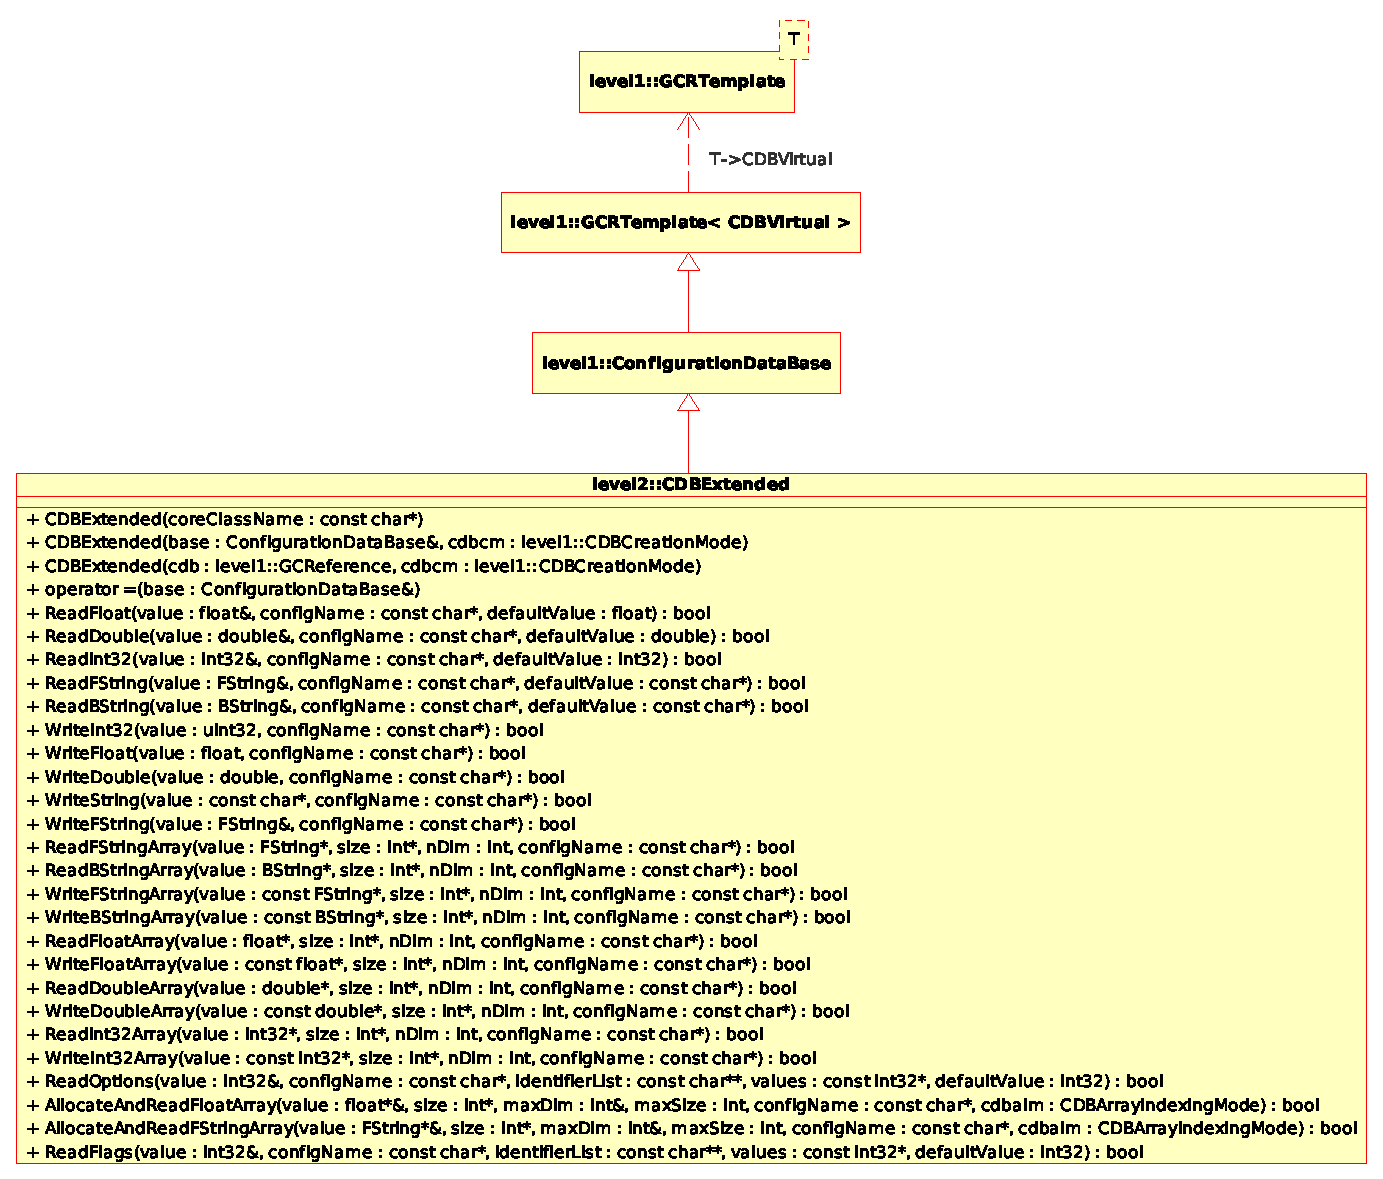
\includegraphics[width=0.83\textwidth]{level2/level2-CDB.eps}
  \caption{BaseLib Level2 CDB classes}
  \label{f:level2:CDB}
 \end{center}
\end{figure}

Basically there is only one class: \texttt{CDBExtended}. This class is an extension to the ConfigurationDataBase class; contains a reference to CDB of type CDBVirtual Forces call to CDB to be made via the virtual table.
Sources, in this group, regarding level2 are:
\begin{itemize}
 \item CDBExtended.h
 \item CDBDataTypes.h
 \item CDBDataTypes.cpp
\end{itemize}

In the following we analyse the \texttt{CDBExtended} class that will simply extends the \texttt{ConfigurationDataBase} with many specialized read and write methods. Such class is written as a collection of inline methods, also constructors are declared as \texttt{inline}.

The first constructor create a CDB from a generic base type, i.e. it will create a new \texttt{CDBNull} and than sets some value. The second constructor if \texttt{base} is specified it creates a new reference to an existing database, \texttt{cdbcm} attribute if is set to \texttt{CDBCM\_CopyAddress} copies the address from the reference. The last constructor is similar to the second one. The copy operator of a CDB creates a new reference to an existing database.\\

\begin{lstlisting}[
extendedchars=true,%
basicstyle=\fontfamily{pcr}\fontseries{m}\selectfont\footnotesize, %
stepnumber=1,%
numberstyle=\tiny,%
keywordstyle=\footnotesize\tt ,%
language=C++]
public:
   inline CDBExtended(const char* coreClassName="CDB")
   inline CDBExtended(ConfigurationDataBase& base,CDBCreationMode cdbcm=CDBCM_CopyAddress);
   inline CDBExtended(GCReference cdb,CDBCreationMode cdbcm=CDBCM_CopyAddress);

   inline void operator=(ConfigurationDataBase& base);
\end{lstlisting}

Next methods address the read and write activity, read methods simply call \texttt{CDBVirtual::ReadArray} and write methods call \texttt{CDBVirtual::WriteArray}. All that with different arguments to read/write \texttt{Float}, \texttt{Double}, \texttt{Int32}, \texttt{FString}, \texttt{BString}, \texttt{FStringArray}, \texttt{BStringArray}, \texttt{FloatArray}, \texttt{DoubleArray} and \texttt{Int32Array}.
\begin{lstlisting}[
extendedchars=true,%
basicstyle=\fontfamily{pcr}\fontseries{m}\selectfont\footnotesize, %
stepnumber=1,%
numberstyle=\tiny,%
keywordstyle=\footnotesize\tt ,%
language=C++]
   inline bool ReadFloat(float &value,const char* configName,float defaultValue = 0);
   inline bool ReadDouble(double &value,const char* configName,double defaultValue = 0);
   inline bool ReadInt32(int32 &value,const char* configName,int32 defaultValue = 0);
   inline bool ReadFString(FString &value,const char* configName,const char *defaultValue = "");
   inline bool ReadBString(BString &value,const char* configName,const char *defaultValue = "");
   inline bool ReadFStringArray(FString* value,int* size,int nDim,const char* configName);
   inline bool ReadBStringArray(BString* value,int* size,int nDim,const char* configName);
   inline bool ReadFloatArray(float* value,int* size,int nDim,const char* configName);
   inline bool ReadDoubleArray(double* value,int* size,int nDim,const char* configName);
   inline bool ReadInt32Array(int32* value,int* size,int nDim,const char* configName);

   inline bool WriteFloat(float value,const char* configName);
   inline bool WriteDouble(double value,const char* configName);
   inline bool WriteInt32(uint32 value,const char* configName);
   inline bool WriteFString(FString &value,const char* configName);
   inline bool WriteString(const char *value,const char* configName);
   inline bool WriteFStringArray(const FString* value,int* size,int nDim,const char* configName);
   inline bool WriteBStringArray(const BString* value,int* size,int nDim,const char* configName);
   inline bool WriteFloatArray(const float* value,int* size,int nDim,const char* configName);
   inline bool WriteDoubleArray(const double* value,int* size,int nDim,const char* configName);
   inline bool WriteInt32Array(const int32* value,int* size,int nDim,const char* configName);
\end{lstlisting}

The method \texttt{ReadOptions} translates an identifier to a value, \texttt{dentifierList} is a zero terminated vector of \texttt{const char*}.
The method \texttt{ReadFlags} translates a vector of identifiers to a bitset value, \texttt{identifierList} is a zero terminated vector of \texttt{const char*} the values associated to each identifier is in \texttt{values}.

The method \texttt{AllocateAndReadFloatArray} finds the matrix dimension first then allocates memory and finally read data; \texttt{size} parameter is a vector of dimensions of size \texttt{maxDim}; \texttt{value} argument will be allocated with at maximum \texttt{maxSize} floats, this routine uses malloc. The method \texttt{AllocateAndReadFStringArray} does exactly the same but handles \texttt{FString} objects; \texttt{value} argument will be allocated with at maximum \texttt{maxSize} \texttt{FString}, this routine used \texttt{new[]}.
\begin{lstlisting}[
extendedchars=true,%
basicstyle=\fontfamily{pcr}\fontseries{m}\selectfont\footnotesize, %
stepnumber=1,%
numberstyle=\tiny,%
keywordstyle=\footnotesize\tt ,%
language=C++]
   inline bool ReadOptions(int32& value,
      const char* configName,
      const char** identifierList,
      const int32* values,
      int32 defaultValue);
   inline bool ReadFlags(int32& value,
      const char* configName,
      const char** identifierList,
      const int32* values,
      int32 defaultValue);

   inline bool AllocateAndReadFloatArray(float*& value,int* size,int& maxDim,int maxSize,
      const char* configName,CDBArrayIndexingMode cdbaim=CDBAIM_Strict);
   inline bool AllocateAndReadFStringArray(FString*& value,int* size,int& maxDim,int maxSize,
      const char* configName,CDBArrayIndexingMode cdbaim=CDBAIM_Strict)
\end{lstlisting}



\subsection{Design Notes}
---



\section{IO devices}
In Level2 there are also two input device classes. Those input devices classes are: the serial line and the keyboard. In Figure \ref{f:level2:Input} the UML schema is depicted.

\begin{figure}[h!]
 \begin{center}
  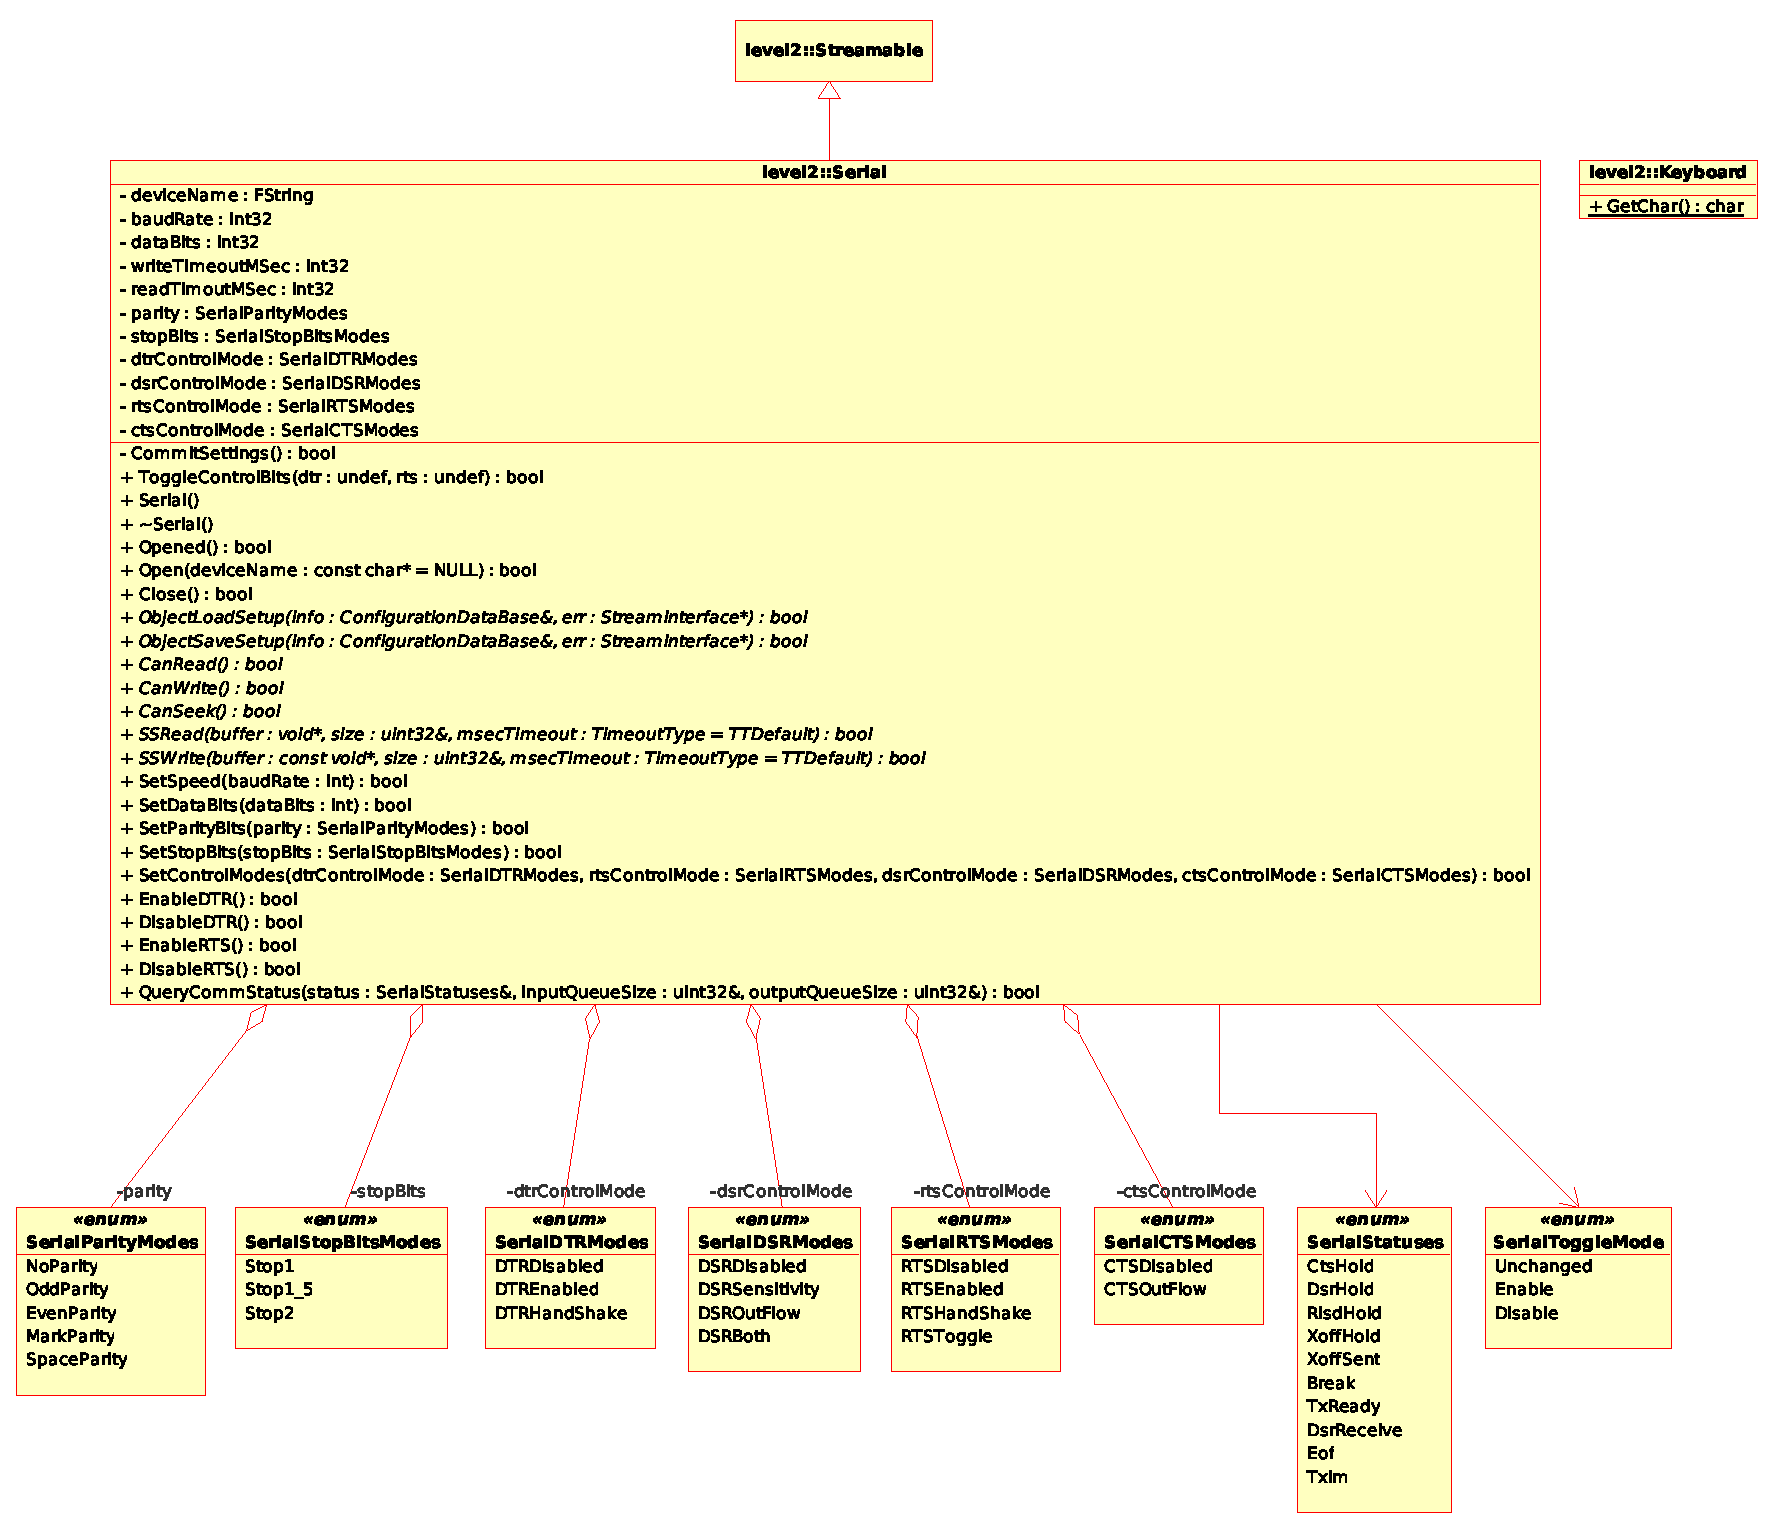
\includegraphics[width=0.83\textwidth]{level2/level2-Input.eps}
  \caption{BaseLib Level2 Input devices classes}
  \label{f:level2:Input}
 \end{center}
\end{figure}

We speak brefily about the \texttt{Keyboard} class than we take a tour of the serial line implementation that is much more interesting and better developed.



\subsubsection{Keyboard}
\texttt{[Keyboard.h]}\\
The \texttt{Keyboard} class manages the direct access to keyboard. The access is done throught a library call, in most UNIX like system the call is \texttt{getchar()}, from the standard C library, in all other system \texttt{\_getch} is used. The result is a read operation of a char without echoing. The straightforward implementation follow.

Note that this class doesn't interface directly with a driver but relay on the Operating System and C libraries.
\begin{lstlisting}[
extendedchars=true,%
basicstyle=\fontfamily{pcr}\fontseries{m}\selectfont\footnotesize, %
stepnumber=1,%
numberstyle=\tiny,%
keywordstyle=\footnotesize\tt ,%
language=C++]
class Keyboard{
public:
#if !(defined(_VXWORKS)||defined(_RTAI)|| defined(_LINUX) || defined(_SOLARIS))
    static  char GetChar() {return _getch();}
#else
    static char GetChar() {return getchar();}
#endif
};
\end{lstlisting}



\subsubsection{Serial}
\texttt{[Serial.h, Serial.cpp]}\\
The class \texttt{Serial} inherits from \texttt{Streamable}, i.e. the serial line can also be treated as a stream of data.\\


The class \texttt{Serial} in some OSes needs a file handle, attribute \texttt{port}, in the class is just defined for OS/2 and Microsoft Windows. The name of the device, the path in some systems, is hold by the \texttt{deviceName} attribute, all other attributes are serial line common properties and settings.
\begin{lstlisting}[
extendedchars=true,%
basicstyle=\fontfamily{pcr}\fontseries{m}\selectfont\footnotesize, %
stepnumber=1,%
numberstyle=\tiny,%
keywordstyle=\footnotesize\tt ,%
language=C++]
#if defined (_OS2)
    HFILE port;
#elif defined (_WIN32)
    HANDLE port;
#endif
   FString deviceName;
   int32 baudRate;
   int32 dataBits;
   int32 writeTimeoutMSec;
   int32 readTimeoutMSec;
   SerialParityModes parity;
   SerialStopBitsModes stopBits;
   SerialDTRModes dtrControlMode;
   SerialDSRModes dsrControlMode;
   SerialRTSModes rtsControlMode;
   SerialCTSModes ctsControlMode;
\end{lstlisting}

The method \texttt{CommitSettings} implements all the programmed changes, some methods only affects class's attributes and calling the method doesn't directly affect the serial line. \texttt{ToggleControlBits} changes the status of \textit{dtr} and \textit{rts} control lines in the serial interface, a value of \texttt{0} means untouched, \texttt{1} means to turn on and \texttt{2} means to turn off.\\


The method \texttt{Opened} query if the serial line device is just opened or not; \texttt{Open} open the device specified in the \texttt{name} argument, the name can be also a path in UNIX, in Microsoft Windows is something like \texttt{COM1}, if \texttt{name} argument is \texttt{NULL} than it will open what was setup using \texttt{ObjectLoadSetup}; \texttt{Close} closes the device.\\


The method \texttt{ObjectLoadSetup} accept from the configuration file the following parameters:
\begin{lstlisting}[
extendedchars=true,%
basicstyle=\fontfamily{pcr}\fontseries{m}\selectfont\footnotesize, %
stepnumber=1,%
numberstyle=\tiny,%
keywordstyle=\footnotesize\tt ,%
language=bash]
   DeviceName COM1:
      BaudRate   int
      DataBits   5 6 7 8 9
      WriteTimeoutMSec   int
      ReadTimeoutMSec   int
      Parity   NoParity OddParity EvenParity MarkParity SpaceParity
      StopBits   Stop1 Stop1_5 Stop2
      RTSControlMode   RTSDisabled RTSEnabled RTSToggle
      DTRControlMode   DTRDisabled DTREnabled DTRHandShake
      DSRControlMode   DSRDisabled DSRSensitivity DSROutFlow DSRBoth
      CTSControlMode   CTSDisabled CTSOutFlow
\end{lstlisting}

The method \texttt{ObjectSaveSetup} is the standard object save function.

Methods\texttt{CanRead} and \texttt{CanWrite} return \texttt{true}; the method \texttt{CanSeek} is not available and return \texttt{false}.
The method \texttt{SSRead} reads a block of data, \texttt{size} is the maximum size, on return \texttt{size} is what was read, the timeout is not supported yet. \texttt{SSWrite} writes a block of data,  \texttt{size} is its size, on return \texttt{size} is what was written.
\begin{lstlisting}[
extendedchars=true,%
basicstyle=\fontfamily{pcr}\fontseries{m}\selectfont\footnotesize, %
stepnumber=1,%
numberstyle=\tiny,%
keywordstyle=\footnotesize\tt ,%
language=C++]
private:
   inline bool CommitSettings();
   inline bool ToggleControlBits(SerialToggleMode dtr, SerialToggleMode rts);

public:
   Serial();
   ~Serial();

   bool Opened();
   bool Open(const char *deviceName=NULL);
   bool Close();

   virtual bool ObjectLoadSetup(ConfigurationDataBase &info,StreamInterface *err);
   virtual bool ObjectSaveSetup(ConfigurationDataBase& info,StreamInterface* err);

   virtual bool CanRead();
   virtual bool CanWrite();
   virtual bool CanSeek();

   virtual bool SSRead(void* buffer,uint32& size,TimeoutType msecTimeout=TTDefault);
   virtual bool Write(const void* buffer,uint32& size,TimeoutType msecTimeout=TTDefault);
\end{lstlisting}

The following function lets the user set the serial line parameters and to enable them.
Last method \texttt{QueryCommStatus} retrieves the status of communication port.
\begin{lstlisting}[
extendedchars=true,%
basicstyle=\fontfamily{pcr}\fontseries{m}\selectfont\footnotesize, %
stepnumber=1,%
numberstyle=\tiny,%
keywordstyle=\footnotesize\tt ,%
language=C++]
   bool SetSpeed(int baudRate);
   bool SetDataBits(int dataBits);
   bool SetParityBits(SerialParityModes parity);
   bool SetStopBits(SerialStopBitsModes stopBits);

   bool SetControlModes(
        SerialDTRModes dtrControlMode,
        SerialRTSModes rtsControlMode,
        SerialDSRModes dsrControlMode,
        SerialCTSModes ctsControlMode);

   inline bool EnableDTR(void);
   inline bool DisableDTR(void);
   inline bool EnableRTS(void);
   inline bool DisableRTS(void);

   inline bool QueryCommStatus(SerialStatuses& status,
      uint32& inputQueueSize,
      uint32& outputQueueSize);
\end{lstlisting}



\subsection{Design Notes}
The class \texttt{Serial} is a \texttt{Streamable} object, but, is not likely to be a real stream of data, it is more an i/o device (why not an IOGAM..) or something architectural dependent, the same can be said for the \texttt{Keyboard} class.

The class \texttt{Keyboard} must be better developed without the need of the C standard library; an architectural dependent keyboard code can be developed to doesn't relay on the OS itself.



